\chapter{Conclusión}

Aprecio que hayas dedicado tiempo a leer este libro y te agradezco por ello. Me motivó a escribirlo el poder ayudarte brindándote el resultado de mi trabajo de investigación sobre Scrum, mi experiencia en proyectos ágiles usando Scrum, mi participación en transformaciones organizacionales hacia la agilidad y de un diálogo constante con profesionales compañeros. 

Para finalizar, después de lo expuesto, quiero concluir que Scrum no es un dogma, ni la solución a los problemas organizacionales. Como mostré, Scrum es un sistema de trabajo flexible para trabajar en contextos de incertidumbre y cambios frecuentes, principalmente en la Industria de Software. Y, si bien se puede aplicar a diversas organizaciones, no significa que resuelva los problemas de cualquiera. Cada empresa con problemas o con intenciones de pasar por transformaciones organizacionales, en busca de ser adaptable y eficiente, tiene sus propias disfuncionalidades que debe analizar y buscar solucionar en su contexto particular. Por otro lado, expuse algunas alternativas de escalamiento y herramientas complementarias para mostrar que, por sí solo, el “núcleo del Sistema Scrum” es insuficiente en organizaciones grandes. Pues, además son necesarias técnicas de XP, Lean, Kanban, System Thinking, Visual Thinking, Game Thinking, etcétera; y sobre todo, aplicar Ingeniería de Software en el desarrollo e Ingeniería de Sistemas en la organización.

El talento de un SM se demuestra facilitando la mejora de las personas, herramientas y procesos en un sistema de trabajo fluyente. La habilidad de un PO se muestra en la búsqueda por lograr, con su equipo, el mejor producto posible para el negocio, satisfaciendo al cliente, y en forma temprana. La excelencia en los desarrolladores es entregar iterativamente, en forma temprana y frecuente, el producto de mejor calidad posible y adaptándose a las necesidades del cliente. La magia de Scrum consiste en no acostumbrarse ni conformarse y siempre avanzar mejorando, en un estado de flujo, con armonía y calidez humana. Haz tu propia experiencia fluyendo con Scrum.

\begin{figure}[h]
  \centering
  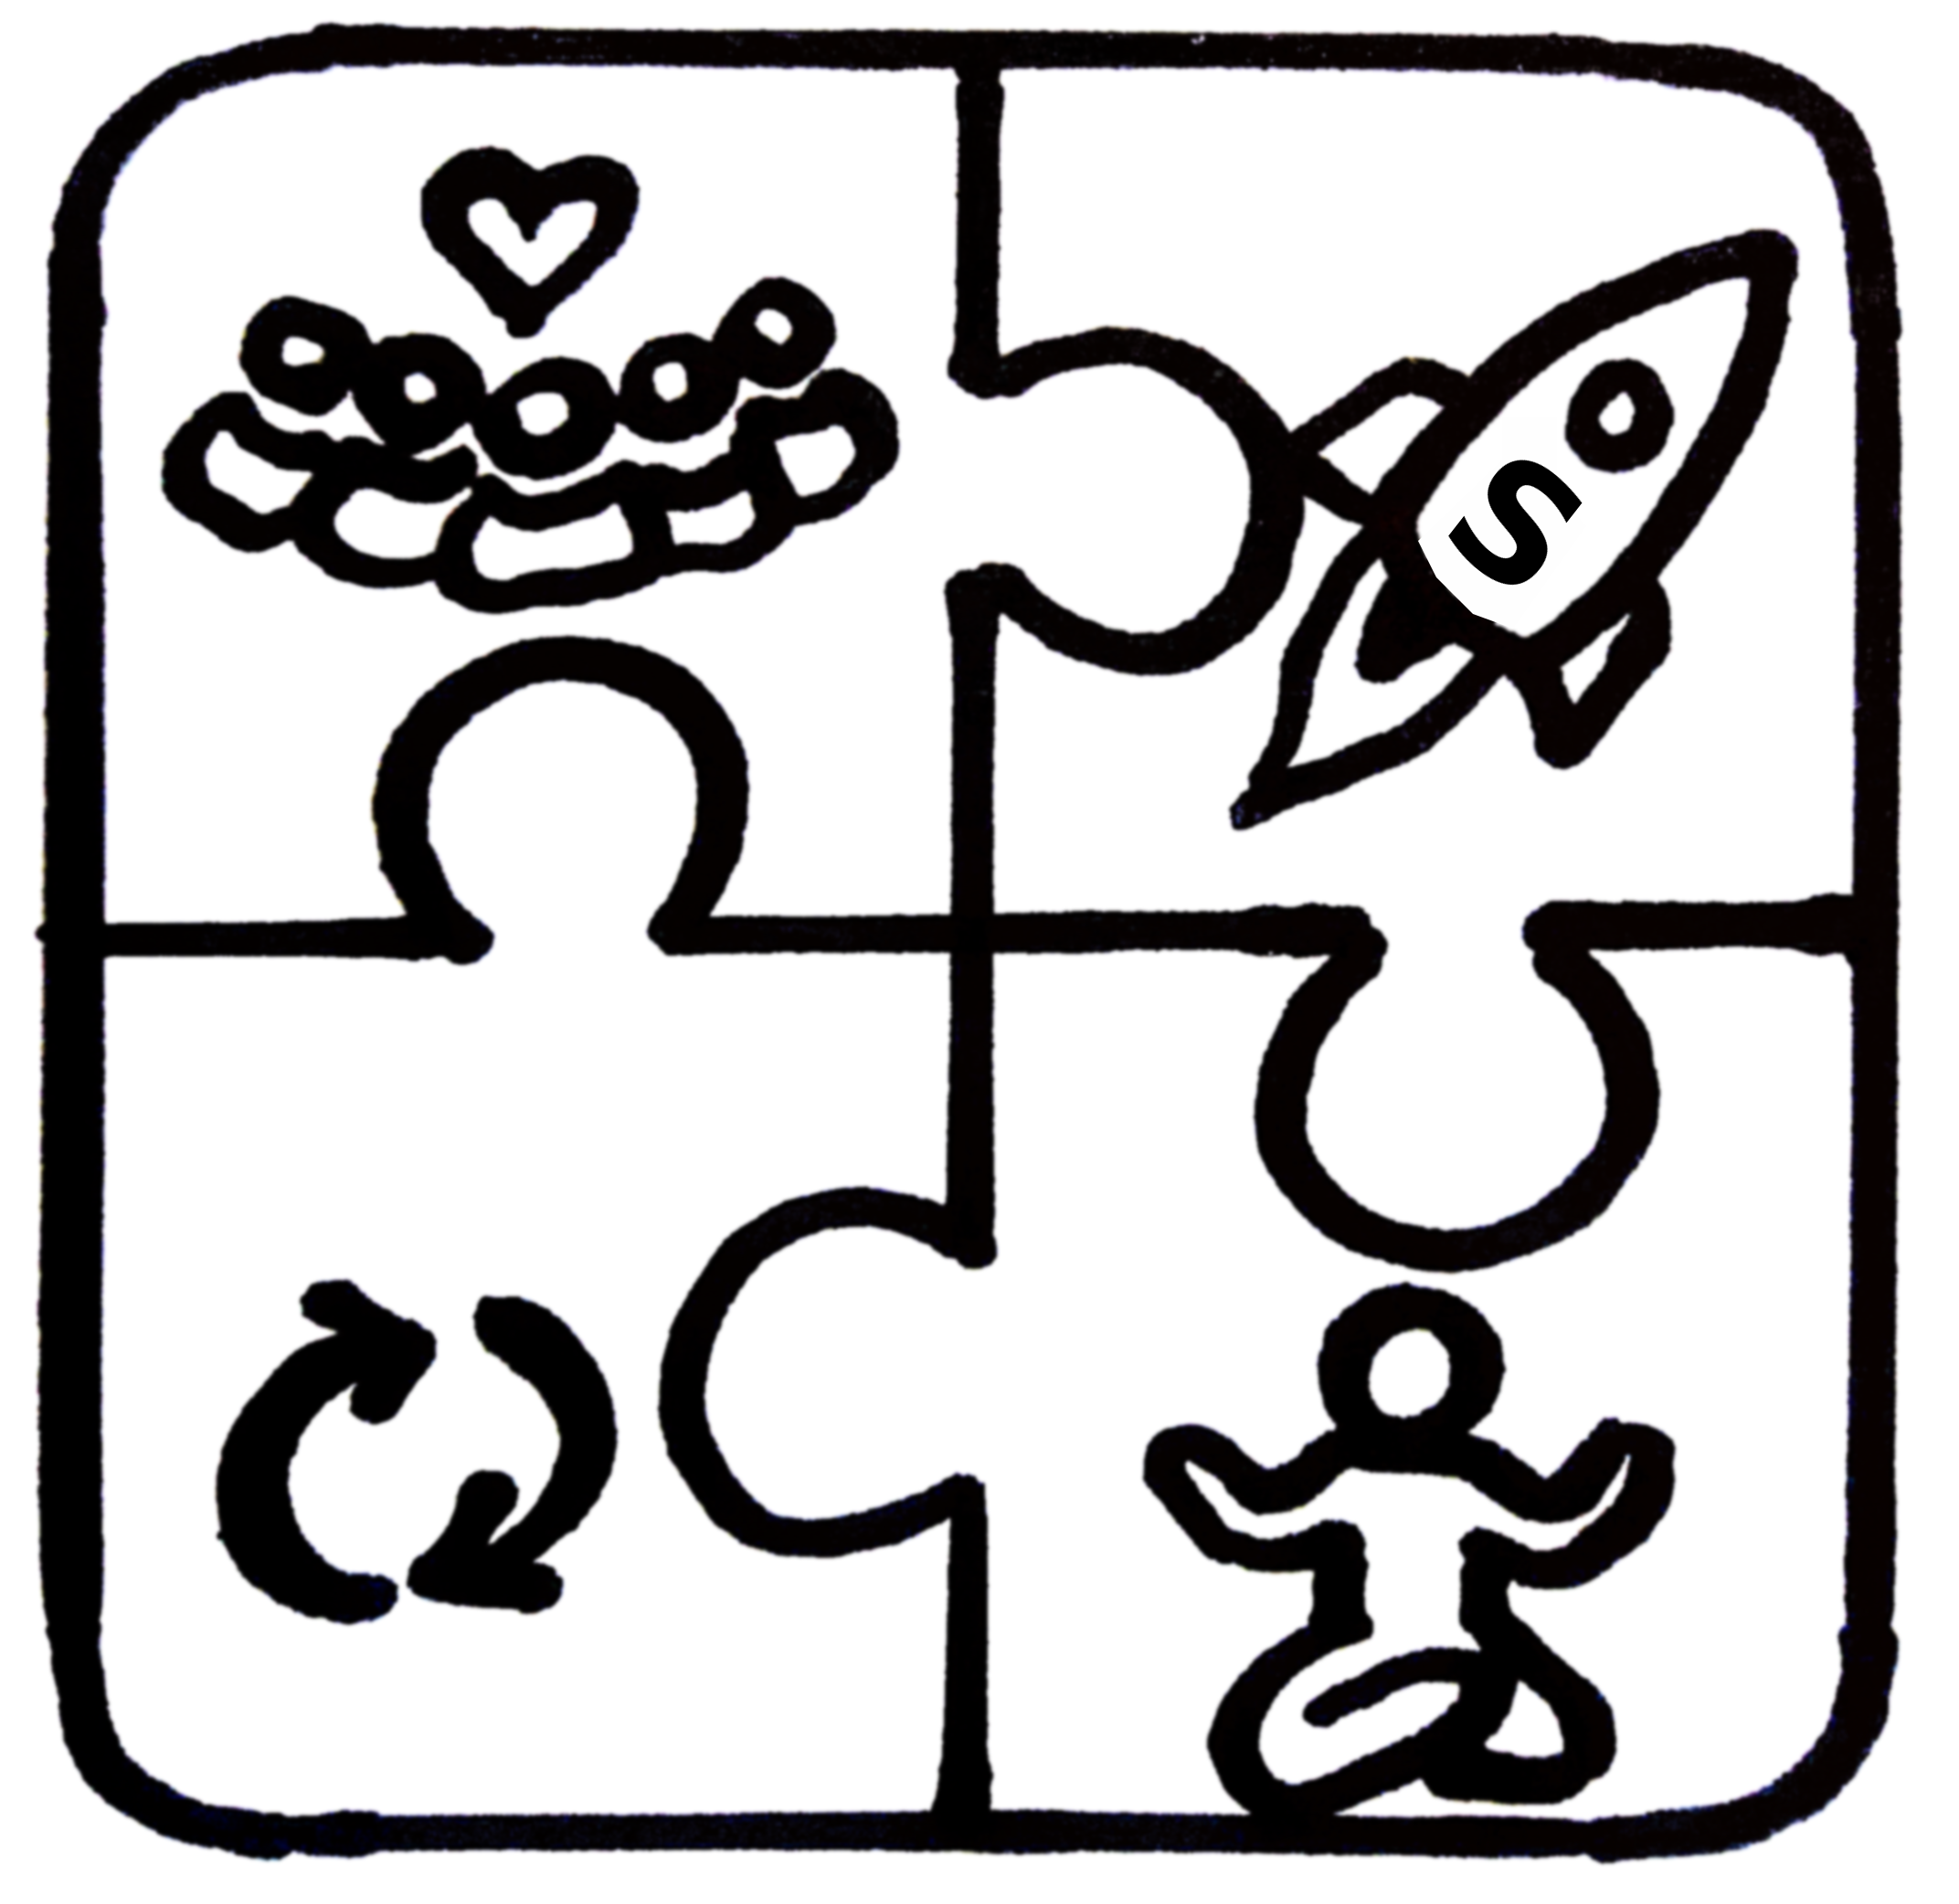
\includegraphics[width=0.50\textwidth]{EmblemaAgil}
  \caption{Emblema ágil}
  \centering
  \label{fig:EmblemaAgil} %\ref{fig:EmblemaAgil}
\end{figure}
